\section{Measured results}
\label{sec:results}
The following values are measurements from the frozen comparison in this study. Table~\ref{tab:direct-times} separates the physical domains and includes completion counts. Summed median times refer only to the matched completed requests.
\begin{table}[!htbp]\centering\small
\caption{Complete times against the preceding application. Done gives preceding/integrated completions. Each domain uses the same requests for both methods.}
\label{tab:direct-times}
\begin{tabularx}{\linewidth}{@{}Yrrrr@{}}\toprule
Domain & Done & Paired & Preceding (s) & Integrated (s)\\\midrule
Two-mass products, 1--13 loops & 13/13 & 13 & 2.271 & 1.935 \\
Connected vacuum trees, 1--13 loops & 34/34 & 34 & 7.900 & 5.719 \\
Zero-invariant tensor bubbles & 3/3 & 3 & 0.577 & 0.569 \\
Ordinary one-loop tensors & 3/3 & 3 & 0.688 & 0.698 \\
Native two-loop boxes & 16/16 & 16 & 100.514 & 100.353 \\
All 69 requests & 69/69 & 69 & 111.950 & 109.273 \\\bottomrule\end{tabularx}\end{table}

On the 69 matched requests, the integrated-to-preceding time ratio is 0.976, with a central 95\% request-resampling interval of $[0.952,0.990]$. The point estimate corresponds to 2.4\% less time. The integrated application is slower on 15 matched requests. This is an incremental comparison with the preceding application on these inputs, rather than a new comparison with unmodified Kira. Earlier percentages use other workloads and cannot be added to this change.

\subsection{Direct formulas and their high-loop scope}
The two-mass product grid changes from 2.271 to 1.935 seconds on 13 matched requests. Direct partial fractions avoid generic one-loop reduction and its preparation for these inputs. The connected vacuum grid changes from 7.900 to 5.719 seconds on 34 matched requests. The connected identity is preserved, while its early dispatch avoids generic symbolic preparation when the simpler tree formula already applies. Both grids contain every loop order from one through thirteen.

The separate analytic coverage grid completes 26 of 26 requests and takes 5.983 seconds in summed median time. Its thirteen repeated-mass requests use an independent symbolic partial-fraction reference, while thirteen coupled massless vacuum requests use the scaleless-integral identity. We report this as exact-domain coverage without assigning a speedup over an unsupported native input. The implementation returns Gamma-function values for the resulting tadpoles and the connected one-mass tree masters, so these domains have an analytic value as well as a decomposition.

The tests contain 14,922 coefficient comparisons across timed outputs. Development additionally checks 48 rational-function identities, 138 product coefficients, 4 native tadpole coefficients, 6 native scaleless target relations, and two convergent radial integrals. These checks test algebra and normalization separately.

\begin{figure}[!htbp]\centering
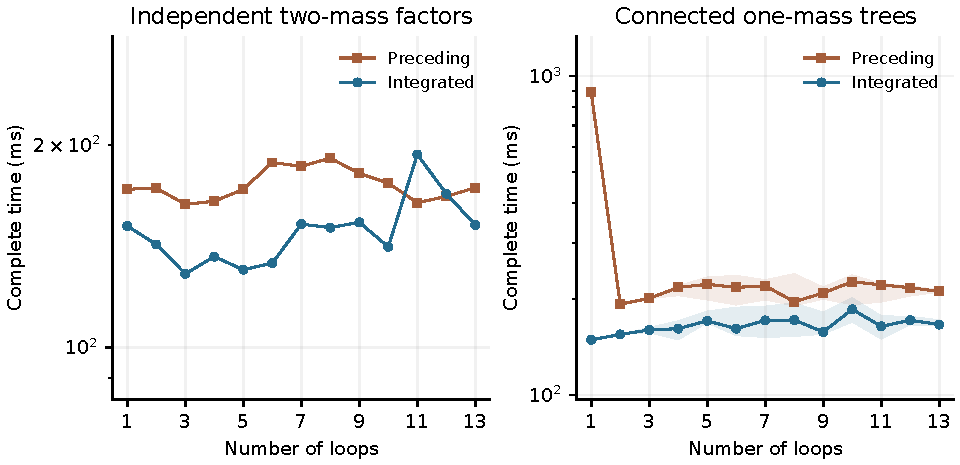
\includegraphics[width=\linewidth]{paper_figures/direct_vacuum.pdf}
\caption{Direct formulas reduce aggregate time in both measured vacuum grids. The panels show complete elapsed time at every tested loop order, with independent factors on the left. In the connected-tree panel, each line gives the median across the tested shapes at that loop order and the shaded band gives their full range. Logarithmic time axes retain the short exact calculations and the slower preparation costs. These domains require the structures stated in the derivations.}
\label{fig:direct-vacuum}
\end{figure}
\subsection{Native seed choices and the ML contribution}
The preliminary ordering experiment verifies all 32 development reductions. Ordering 1 has the lowest sum of development times, so the final native actions retain it. The subsequent model chooses the seed procedure. Validation selects 1 cost tree with maximum depth 1 and a minimum leaf population of 2. Its fixed control is the tight sparse region. The selected validation cost is 86.114 seconds, including the prediction allowance and failure penalties; the fixed control gives 86.090 seconds. Validation rejects the replacement because the deployment condition is not met. The final application retains the preceding validated native seed model.

On the 16 matched reserved native batches, the fixed application takes 100.166 seconds and the integrated application takes 100.353 seconds. Their ratio is 1.002, with interval $[0.994,1.012]$. This interval includes equal time and does not resolve a consistent additional learned saving. The integrated method is slower on 7 matched batches. The retained native policy changes the fixed action on 0 of the sixteen requests in the final repetition. Thus the retained model selects the fixed action throughout this final sample; the measured difference includes prediction overhead and run-to-run variation, and supplies no additional learned speedup. Median measured model loading and decision time is 2.661 milliseconds. Exact formulas, the native interface, and recovery checks are shared by the learned and fixed controls.

Across 48 native applications per method, unverified output counts are 0 for the integrated application, 0 for the fixed control, and 0 for the preceding application. Recorded failed inner attempts total 0, 0, and 0, respectively. A terminated application can lack an inner-attempt record and remains in the separate application-failure count. Complete-region selection can avoid a sparse failure, but these measurements do not guarantee success for unseen inputs.

\begin{figure}[!htbp]\centering
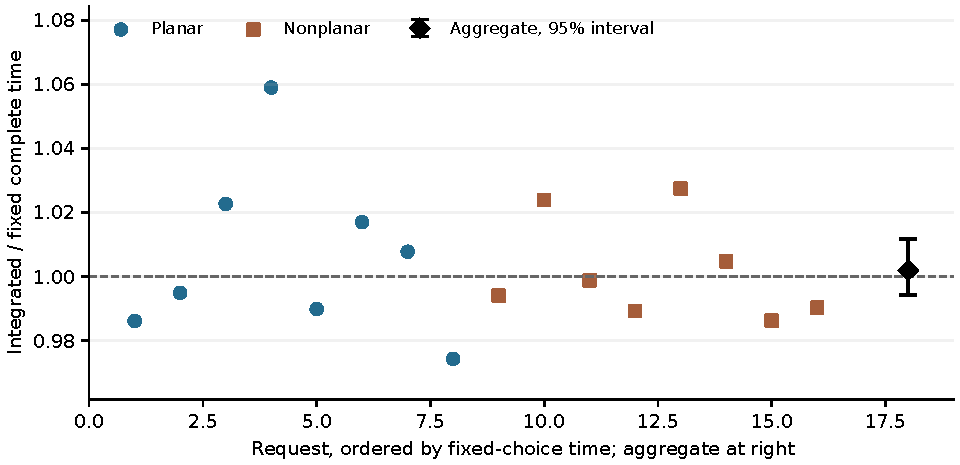
\includegraphics[width=.96\linewidth]{paper_figures/direct_native.pdf}
\caption{The retained model chooses the fixed action on every final batch, so this sample demonstrates no additional ML saving. Both controls use the same exact methods and native implementation. Points below one indicate a lower measured integrated time. Individual batches show variation, while the aggregate point reports the ratio of summed median times and its request-resampling interval.}
\label{fig:direct-native}
\end{figure}
\subsection{The other learned interventions}
Table~\ref{tab:retained-results} retains the main earlier controls needed to interpret the method. They use different workloads and cannot be multiplied into a cumulative speed factor. The equation-filter result supports that intervention on its tested domain, while the row results motivate its omission. The current combined experiment keeps equation filtering off and does not claim a joint seed-plus-equation gain.
\begin{table}[!htbp]\centering\small
\caption{Earlier measurements from this study, retained as separate evidence. A ratio below one means less time. Their full input definitions and measurements remain in the notes.}
\label{tab:retained-results}
\begin{tabularx}{\linewidth}{@{}YYr@{}}\toprule
Intervention & Control and workload & Time ratio\\\midrule
Earlier native seed model & Fixed region, 32 box batches: 156.383 to 150.663 s & 0.963\\
Equation selection & Native filter, 24 new-index batches: 72.295 to 67.478 s & 0.933\\
Original learned row model & Native row choices, 84 trials & 1.305\\
Compiled row-cost policy & Native row choices; geometric mean & 0.982\\\bottomrule
\end{tabularx}
\end{table}
The earlier seed comparison has interval $[0.937,0.984]$, and the equation comparison has interval $[0.928,0.940]$. The compiled row policy has interval $[0.959,1.003]$, which includes equal time. These intervals use the resampling procedure recorded for each original study. The native row algorithm remains in the retained workflow.

\subsection{Scope of the result}
The direct formulas prove reductions and analytic values within their stated domains. The test covers every loop order through thirteen for independent vacuum products and connected one-mass trees. The native test covers new target batches and kinematic points within two known two-loop scattering graphs. General coupled multiscale scattering at every loop order remains outside this evidence. Loop count alone does not classify the difficulty or determine whether a particular exact rule applies.

The controls separate changes in the integrated application from the additional effect of learned selection. A finite search over models and native settings cannot establish globally minimum time for every integral. The retained measurements include slower requests, unsuccessful attempts, and incomplete applications so that these limits remain part of the result.
\FloatBarrier
